\chapter{Cellular Respiration}\label{ch:g10:cellular-respiration}

Sugars store energy; life spends it as \omterm{def:g10:cellular-respiration:ATP}{ATP}. \omterm{def:g10:cellular-respiration:def}{Cellular respiration} unlocks
energy from organic molecules in a controlled \omterm{def:g10:molecules-of-life:proteins}{sequence} --- not a single
explosion --- so \omterm{def:g10:the-cell:cell}{cells} can power pumps, synthesis and movement. This
chapter maps the pathway from glucose to $\mathrm{CO_2}$ and
$\mathrm{H_2O}$, places it in the \omterm{def:g10:cellular-respiration:mito}{mitochondrion}, and links it to
\omterm{def:g10:photosynthesis:def}{photosynthesis} as the other half of the carbon--energy cycle.

\section{Energy currency}

\begin{definition}[ATP]\label{def:g10:cellular-respiration:ATP}
\emph{Adenosine triphosphate}\index{ATP} (ATP) is the \omterm{def:g10:the-cell:cell}{cell}'s immediate
energy currency. \omterm{def:g10:molecules-of-life:polymer}{Hydrolysis} of ATP to ADP + phosphate releases free
energy that drives endergonic work. ATP is constantly regenerated from
ADP.
\end{definition}

\begin{definition}[Cellular respiration]\label{def:g10:cellular-respiration:def}
\emph{Cellular respiration}\index{cellular respiration} is the
enzyme-catalysed oxidation of organic fuels (often glucose) to harvest
energy for \omterm{def:g10:cellular-respiration:ATP}{ATP} synthesis. \emph{Aerobic respiration}\index{aerobic
respiration} uses oxygen as the final electron acceptor;
\emph{anaerobic}\index{anaerobic respiration} pathways and \omterm{def:g10:cellular-respiration:ferment}{fermentation}
operate without oxygen and yield far less \omterm{def:g10:cellular-respiration:ATP}{ATP} per glucose.
\end{definition}

\begin{proposition}[Overall aerobic equation]\label{prop:g10:cellular-respiration:equation}
\[
\mathrm{C_6H_{12}O_6} + 6\,\mathrm{O_2}
\to
6\,\mathrm{CO_2} + 6\,\mathrm{H_2O} + \text{energy (ATP + heat)}.
\]
Compare with \omterm{def:g10:photosynthesis:def}{photosynthesis} (\cref{ch:g10:photosynthesis}): the equations
are reverse in outline, but the pathways and \omterm{def:g10:the-cell:prok-euk}{organelles} differ.
\end{proposition}
\admitted

\section{Stages of aerobic respiration}

\begin{definition}[Glycolysis]\label{def:g10:cellular-respiration:glycolysis}
\emph{Glycolysis}\index{glycolysis} occurs in the cytosol: one glucose
(6C) is split into two pyruvate (3C), with a small net yield of \omterm{def:g10:cellular-respiration:ATP}{ATP} and
reduced NAD (NADH). Oxygen is not required for glycolysis itself.
\end{definition}

\begin{definition}[Link reaction and Krebs cycle]\label{def:g10:cellular-respiration:krebs}
In the mitochondrial \omterm{def:g10:cellular-respiration:mito}{matrix}, pyruvate is converted to acetyl-CoA
(releasing $\mathrm{CO_2}$). The \emph{Krebs cycle}\index{Krebs cycle}
(citric acid cycle) oxidises acetyl groups to $\mathrm{CO_2}$, generating
more NADH/FADH$_2$ and a little \omterm{def:g10:cellular-respiration:ATP}{ATP} (or GTP).
\end{definition}

\begin{definition}[Electron transport chain]\label{def:g10:cellular-respiration:ETC}
On the inner mitochondrial membrane, the \emph{electron transport
chain}\index{electron transport chain} (ETC) transfers electrons from
NADH/FADH$_2$ to $\mathrm{O_2}$, forming water. Energy released pumps
protons; their flow back through \omterm{def:g10:cellular-respiration:ATP}{ATP} synthase makes most of the \omterm{def:g10:cellular-respiration:ATP}{ATP}
(\emph{oxidative phosphorylation}\index{oxidative phosphorylation}).
\end{definition}

\begin{omfigure}
\begin{tikzpicture}[font=\footnotesize,
  box/.style={draw, rounded corners, minimum width=2.3cm,
    minimum height=0.85cm, align=center}]
  \node[box, fill=omDef!12] (g) at (0,0) {glycolysis\\(cytosol)};
  \node[box, fill=omProp!12] (k) at (3.6,0) {Krebs\\(matrix)};
  \node[box, fill=omThm!12] (e) at (7.2,0) {ETC\\(inner mem.)};
  \draw[-Stealth, thick] (g) -- (k);
  \draw[-Stealth, thick] (k) -- (e);
  \draw[-Stealth, thick] (-2.0,0) -- (g)
    node[midway, above] {glucose};
  \draw[-Stealth, thick, omMeth] (e.east) -- ++(1.1,0)
    node[right] {ATP};
  \draw[-Stealth, omExo] (k.south) -- ++(0,-0.55)
    node[below] {$\mathrm{CO_2}$};
  \draw[-Stealth, omExo] (e.south) -- ++(0,-0.55)
    node[below] {$\mathrm{H_2O}$};
  \node[omThm] at (7.2,1.0) {$\mathrm{O_2}$ in};
\end{tikzpicture}

{\small Three-stage map of \omterm{def:g10:cellular-respiration:def}{aerobic respiration}: small \omterm{def:g10:cellular-respiration:ATP}{ATP} early; bulk
\omterm{def:g10:cellular-respiration:ATP}{ATP} at the ETC when oxygen accepts electrons.}
\end{omfigure}

\begin{example}[Yield order of magnitude]\label{ex:g10:cellular-respiration:yield}
Per glucose, \omterm{def:g10:cellular-respiration:glycolysis}{glycolysis} + Krebs produce only a few \omterm{def:g10:cellular-respiration:ATP}{ATP} directly; \omterm{def:g10:cellular-respiration:ETC}{oxidative
phosphorylation} multiplies the harvest (commonly summarised near
$\sim 30$ \omterm{def:g10:cellular-respiration:ATP}{ATP} per glucose in textbooks, with real yields varying). Without
oxygen, the ETC stops and only glycolytic \omterm{def:g10:cellular-respiration:ATP}{ATP} remains available via
\omterm{def:g10:cellular-respiration:ferment}{fermentation} routes.
\end{example}

\section{The mitochondrion}

\begin{definition}[Mitochondrial structure]\label{def:g10:cellular-respiration:mito}
A \emph{mitochondrion}\index{mitochondrion} has a smooth outer membrane
and a folded inner membrane (\emph{cristae}\index{cristae}) that increase
\omterm{def:g10:the-cell:sa-v}{surface area} for ETC complexes and \omterm{def:g10:cellular-respiration:ATP}{ATP} synthase. The
\emph{matrix}\index{matrix (mitochondrion)} holds Krebs \omterm{def:g10:membranes-enzymes:enzyme}{enzymes} and
mitochondrial \omterm{def:g10:molecules-of-life:nucleic}{DNA}.
\end{definition}

\begin{omfigure}
\begin{tikzpicture}[font=\footnotesize]
  \draw[thick, omDef, fill=omDef!8] (0,0) ellipse (3.3 and 1.5);
  \draw[thick, omThm, fill=omThm!10] (0,0) ellipse (2.85 and 1.15);
  \draw[thick, omThm]
    (-1.8,0) .. controls (-1.2,0.7) and (-0.4,0.7) .. (0.2,0)
    .. controls (0.8,-0.7) and (1.6,-0.7) .. (2.2,0);
  \node[omProp] at (0,0.2) {matrix};
  \node[omThm] at (1.0,0.85) {crista};
  \node at (0,-1.9) {mitochondrion (schematic)};
\end{tikzpicture}

{\small \omterm{def:g10:cellular-respiration:mito}{Cristae} expand the inner membrane: more room for the ETC and \omterm{def:g10:cellular-respiration:ATP}{ATP}
synthase.}
\end{omfigure}

\section{Fermentation}

\begin{definition}[Fermentation]\label{def:g10:cellular-respiration:ferment}
\emph{Fermentation}\index{fermentation} regenerates NAD$^+$ from NADH so
\omterm{def:g10:cellular-respiration:glycolysis}{glycolysis} can continue when the ETC is unavailable. Net \omterm{def:g10:cellular-respiration:ATP}{ATP} per glucose is
only the small glycolytic yield (classically $2$ \omterm{def:g10:cellular-respiration:ATP}{ATP}), because the \omterm{def:g10:cellular-respiration:krebs}{Krebs cycle}
and \omterm{def:g10:cellular-respiration:ETC}{oxidative phosphorylation} do not run.
\end{definition}

\begin{definition}[Lactic acid fermentation]
\label{def:g10:cellular-respiration:lactic}
In \emph{lactic acid fermentation}\index{lactic acid fermentation}, pyruvate
is reduced to \emph{lactate}\index{lactate} (lactic acid), oxidising NADH to
NAD$^+$. Human skeletal muscle uses this pathway during intense effort when
oxygen delivery lags \omterm{def:g10:cellular-respiration:ATP}{ATP} demand; some bacteria (e.g.\ in yoghurt) do the same.
\end{definition}

\begin{definition}[Alcoholic fermentation]
\label{def:g10:cellular-respiration:alcoholic}
In \emph{alcoholic fermentation}\index{alcoholic fermentation} (typical of
yeast), pyruvate is converted to \emph{ethanol}\index{ethanol} and
$\mathrm{CO_2}$, again regenerating NAD$^+$. Bakers exploit the gas for
rising dough; brewers keep the ethanol.
\end{definition}

\begin{proposition}[Lactic vs alcoholic]\label{prop:g10:cellular-respiration:ferm-compare}
Both pathways start from glycolytic pyruvate and exist to recycle NAD$^+$.
They differ in end products (\omterm{def:g10:cellular-respiration:lactic}{lactate} versus \omterm{def:g10:cellular-respiration:alcoholic}{ethanol} + $\mathrm{CO_2}$) and in
which \omterm{def:g10:scientific-biology:organism}{organisms} use them routinely. Neither oxidises fuel fully to
$\mathrm{CO_2}$ and $\mathrm{H_2O}$, so both waste most of the chemical energy
still stored in the organic end product.
\end{proposition}
\admitted

\begin{example}[Sprint then recovery]\label{ex:g10:cellular-respiration:muscle}
During a short sprint, muscle \omterm{def:g10:cellular-respiration:ATP}{ATP} turnover soars. \omterm{def:g10:cellular-respiration:glycolysis}{Glycolysis} accelerates;
when oxygen cannot keep the ETC fast enough, \omterm{def:g10:cellular-respiration:lactic}{lactate} \omterm{def:g10:cellular-respiration:ferment}{fermentation} keeps NAD$^+$
available so some \omterm{def:g10:cellular-respiration:ATP}{ATP} continues. After the race, breathing rate stays high
while the body restores oxygen stores, clears \omterm{def:g10:cellular-respiration:lactic}{lactate} and rebuilds \omterm{def:g10:cellular-respiration:ATP}{ATP} and
creatine phosphate --- the so-called oxygen debt or recovery \omterm{def:g10:scientific-biology:properties}{metabolism}.
\end{example}

\begin{omfigure}
\begin{tikzpicture}[font=\footnotesize,
  box/.style={draw, rounded corners, minimum width=2.0cm,
    minimum height=0.7cm, align=center}]
  \node[box, fill=omDef!12] (g) at (0,0) {glucose};
  \node[box, fill=omMeth!12] (p) at (3.2,0) {pyruvate};
  \node[box, fill=omProp!12] (lac) at (6.4,1.0) {lactate};
  \node[box, fill=omThm!12] (eth) at (6.4,-1.0) {ethanol + $\mathrm{CO_2}$};
  \draw[-Stealth, thick] (g) -- (p) node[midway, above] {glycolysis};
  \draw[-Stealth, thick] (p) -- (lac)
    node[midway, above, sloped, font=\scriptsize] {muscle/bacteria};
  \draw[-Stealth, thick] (p) -- (eth)
    node[midway, below, sloped, font=\scriptsize] {yeast};
  \node[align=left] at (3.2,-1.7) {both regenerate NAD$^+$\\for more glycolysis};
\end{tikzpicture}

{\small Two \omterm{def:g10:cellular-respiration:ferment}{fermentation} branches from pyruvate. The purpose is NAD$^+$
recycling, not maximising \omterm{def:g10:cellular-respiration:ATP}{ATP}.}
\end{omfigure}

\begin{omfigure}
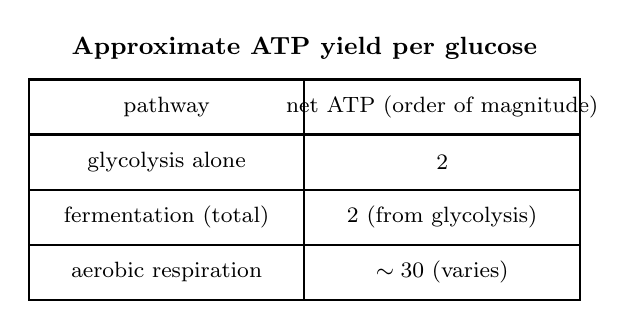
\begin{tikzpicture}[font=\small]
  \node[align=center] at (3.5,3.2) {\textbf{Approximate ATP yield per glucose}};
  % table-like boxes
  \draw[thick] (0,0) rectangle (7,2.8);
  \draw[thick] (0,2.1) -- (7,2.1);
  \draw[thick] (0,1.4) -- (7,1.4);
  \draw[thick] (0,0.7) -- (7,0.7);
  \draw[thick] (3.5,0) -- (3.5,2.8);
  \node[font=\footnotesize, align=center] at (1.75,2.45) {pathway};
  \node[font=\footnotesize, align=center] at (5.25,2.45) {net ATP (order of magnitude)};
  \node[font=\footnotesize, align=center] at (1.75,1.75) {glycolysis alone};
  \node[font=\footnotesize, align=center] at (5.25,1.75) {$2$};
  \node[font=\footnotesize, align=center] at (1.75,1.05) {fermentation (total)};
  \node[font=\footnotesize, align=center] at (5.25,1.05) {$2$ (from glycolysis)};
  \node[font=\footnotesize, align=center] at (1.75,0.35) {aerobic respiration};
  \node[font=\footnotesize, align=center] at (5.25,0.35) {$\sim 30$ (varies)};
\end{tikzpicture}

{\small \omterm{def:g10:cellular-respiration:ATP}{ATP} bookkeeping: \omterm{def:g10:cellular-respiration:ferment}{fermentation} matches \omterm{def:g10:cellular-respiration:glycolysis}{glycolysis} only; aerobic
oxidation multiplies the harvest when oxygen accepts electrons at the ETC.}
\end{omfigure}

\begin{remark}[Not the opposite of breathing]\label{rem:g10:cellular-respiration:breathing}
``Respiration'' in \omterm{def:g10:scientific-biology:science}{biology} means cellular energy pathways. Breathing
(ventilation) only supplies $\mathrm{O_2}$ and removes $\mathrm{CO_2}$
for aerobic \omterm{def:g10:scientific-biology:organism}{organisms} --- necessary support, not the same process.
\end{remark}

\section{Link to photosynthesis}

\begin{proposition}[A cycle of carbon and energy]\label{prop:g10:cellular-respiration:link}
\omterm{def:g10:photosynthesis:def}{Photosynthesis} stores light energy in organic molecules and releases
$\mathrm{O_2}$. Respiration releases that chemical energy as \omterm{def:g10:cellular-respiration:ATP}{ATP} (and
heat) and returns $\mathrm{CO_2}$ and $\mathrm{H_2O}$. In the biosphere
the two couple; in a plant \omterm{def:g10:the-cell:cell}{cell} both can run (\omterm{def:g10:photosynthesis:chloroplast}{chloroplasts} and
mitochondria).
\end{proposition}
\admitted

\begin{omfigure}
\begin{tikzpicture}[font=\small,
  box/.style={draw, rounded corners, fill=omDef!12, minimum width=2.8cm,
    minimum height=1.0cm, align=center}]
  \node[box] (p) at (0,1.2) {photosynthesis};
  \node[box, fill=omThm!12] (r) at (0,-1.2) {respiration};
  \draw[-Stealth, thick, omMeth] (1.6,1.0) arc (-60:60:1.4)
    node[midway, right, font=\footnotesize] {$\mathrm{O_2}$, sugars};
  \draw[-Stealth, thick, omProp] (-1.6,-1.0) arc (120:240:1.4)
    node[midway, left, font=\footnotesize] {$\mathrm{CO_2}$, $\mathrm{H_2O}$};
  \draw[-Stealth, omDef] (0,2.4) -- (p)
    node[midway, right, font=\footnotesize] {light};
  \draw[-Stealth, omThm] (r) -- (0,-2.4)
    node[midway, right, font=\footnotesize] {ATP + heat};
\end{tikzpicture}

{\small Global coupling: energy enters as light and leaves as heat; matter
cycles as $\mathrm{CO_2}$, $\mathrm{H_2O}$ and organics.}
\end{omfigure}

\section{Exercises}

\begin{exercise}[$\star$]\label{exo:g10:cellular-respiration:1}
Write the balanced overall equation for \omterm{def:g10:cellular-respiration:def}{aerobic respiration} of glucose.
Where does the released energy go?
\end{exercise}

\begin{exercise}[$\star$]\label{exo:g10:cellular-respiration:2}
Name the three main stages of \omterm{def:g10:cellular-respiration:def}{aerobic respiration} and their locations in
a \omterm{def:g10:the-cell:prok-euk}{eukaryotic cell}.
\end{exercise}

\begin{exercise}[$\star$]\label{exo:g10:cellular-respiration:3}
What is the role of oxygen in \omterm{def:g10:cellular-respiration:def}{aerobic respiration}?
\end{exercise}

\begin{exercise}[$\star$]\label{exo:g10:cellular-respiration:4}
Why is \omterm{def:g10:cellular-respiration:ATP}{ATP} described as an energy ``currency'' rather than a long-term
store?
\end{exercise}

\begin{exercise}[$\star$]\label{exo:g10:cellular-respiration:5}
Compare \omterm{def:g10:cellular-respiration:def}{aerobic respiration} and \omterm{def:g10:cellular-respiration:ferment}{fermentation}: oxygen need, relative \omterm{def:g10:cellular-respiration:ATP}{ATP}
yield, and one product of each \omterm{def:g10:cellular-respiration:ferment}{fermentation} type named in the chapter.
\end{exercise}

\begin{exercise}[$\star\star$]\label{exo:g10:cellular-respiration:6}
Explain why cyanide, which blocks the \omterm{def:g10:cellular-respiration:ETC}{electron transport chain}, is lethal
to aerobic \omterm{def:g10:scientific-biology:organism}{organisms} even if glucose is abundant.
\end{exercise}

\begin{exercise}[$\star\star$]\label{exo:g10:cellular-respiration:7}
Muscle \omterm{def:g10:the-cell:cell}{cells} during a sprint produce \omterm{def:g10:cellular-respiration:lactic}{lactate}. Why does \omterm{def:g10:cellular-respiration:glycolysis}{glycolysis} need
\omterm{def:g10:cellular-respiration:ferment}{fermentation} under low oxygen, in terms of NAD$^+$?
\end{exercise}

\begin{exercise}[$\star\star$]\label{exo:g10:cellular-respiration:8}
How do \omterm{def:g10:cellular-respiration:mito}{cristae} relate to the surface-to-volume idea from
\cref{ch:g10:the-cell}?
\end{exercise}

\begin{exercise}[$\star\star$]\label{exo:g10:cellular-respiration:9}
A seed germinates in the dark and loses dry mass for several days. Explain
using respiration and the absence of \omterm{def:g10:photosynthesis:def}{photosynthesis}.
\end{exercise}

\begin{exercise}[$\star\star\star$]\label{exo:g10:cellular-respiration:10}
Design a respirometer (or simple CO$_2$/O$_2$ indicator) \omterm{def:g10:scientific-biology:experiment}{experiment} to
compare respiration rate of germinating seeds at two temperatures. List
variables and a control.
\end{exercise}

\begin{exercise}[$\star\star\star$]\label{exo:g10:cellular-respiration:11}
Trace a carbon atom from $\mathrm{CO_2}$ in the air to a starch grain in
a leaf, then to $\mathrm{CO_2}$ exhaled by an animal that ate the plant.
Name the key processes at each step.
\end{exercise}

\begin{exercise}[$\star\star$]\label{exo:g10:cellular-respiration:12}
Compare \omterm{def:g10:cellular-respiration:lactic}{lactic acid fermentation} and \omterm{def:g10:cellular-respiration:alcoholic}{alcoholic fermentation}: \omterm{def:g10:scientific-biology:organism}{organism}
examples, end products, and shared purpose regarding NAD$^+$. Why is the
\omterm{def:g10:cellular-respiration:ATP}{ATP} yield of either pathway so low compared with \omterm{def:g10:cellular-respiration:def}{aerobic respiration}?
\end{exercise}

\begin{exercise}[$\star\star\star$]\label{exo:g10:cellular-respiration:13}
A student claims that after a $100\,\mathrm{m}$ sprint, high breathing
rate ``pays back oxygen that was used to make \omterm{def:g10:cellular-respiration:lactic}{lactate}.'' Correct and
improve this statement using \omterm{def:g10:cellular-respiration:glycolysis}{glycolysis}, NAD$^+$, and recovery
\omterm{def:g10:scientific-biology:properties}{metabolism}.
\end{exercise}

\section{Problem: Marathon of a molecule}

\begin{problem}[{Weekend problem --- follow glucose from gut to
mitochondrion: stages, ATP logic and the photosynthesis link}]
\label{pb:g10:cellular-respiration:1}
After a pasta meal, glucose reaches muscle \omterm{def:g10:the-cell:cell}{cells} that are exercising
steadily with good oxygen supply, then later briefly with oxygen debt.

\medskip
\noindent\textbf{Part I --- Aerobic path.}
\begin{enumerate}
  \item List the stages from glucose to water, naming sites.
  \item At which stage is most \omterm{def:g10:cellular-respiration:ATP}{ATP} made? What molecule accepts electrons
        at the end of the ETC?
\end{enumerate}

\medskip
\noindent\textbf{Part II --- Oxygen debt.}
\begin{enumerate}
  \item What pathway keeps some \omterm{def:g10:cellular-respiration:ATP}{ATP} production going when oxygen delivery
        lags?
  \item Why can this not sustain the same power output as aerobic
        \omterm{def:g10:scientific-biology:properties}{metabolism}?
\end{enumerate}

\medskip
\noindent\textbf{Part III --- Big picture.}
\begin{enumerate}
  \item Write \omterm{def:g10:photosynthesis:def}{photosynthesis} and respiration equations side by side and
        circle the shared molecules.
  \item Explain why a plant in continuous darkness still needs
        mitochondria.
\end{enumerate}
\end{problem}
